\section{Zielsetzung}
Ziel dieses Versuches ist es, den Zerfall von $\beta$- und $\gamma$-Strahlung zu untersuchen.
Zusätzlich soll die maximale Energie der $\beta$-Strahlung bestimmt werden, während
aus den Ergebnissen für die $\gamma$-Strahlung Rückschlüsse über den vorliegenden
Absorptionsmechanismus gezogen werden sollen.

\section{Theorie}
\label{sec:Theorie}

Trifft ein Teilchenstrahl auf Materie, so treten Wechselwirkungen mit den einzelnen Bausteinen dieser
Materie auf. Dies führt im allgemeinen zu einer Intensitätsabnahme des Strahls.
Um die Häufigkeit der verschiedenen Wechselwirkungen zu beschreiben, eignet sich der sogenannte
Wirkungsquerschnitt $\sigma$.
Mit ihm lässt sich die Wahrscheinlichkeit $W$, dass ein Teilchen mit einem Absorber mit Querschnitt $F$,
Dicke $D$ und $n$ Materieteilchen pro Volumen wechselwirkt schreiben als
\begin{equation}
    \label{sigma}
    W=\frac{nFD\sigma}{F}=nD\sigma.
\end{equation}
Wird angenommen, dass die Elektronen des Absorbers die Wechselwirkungszentren darstellen, dann gilt
\begin{equation}
    \label{n}
    n=\frac{Z N_{\symup{L}} \rho}{M}
\end{equation}
wobei $Z$ die Ordnungszahl, $N_{\symup{L}}$ die Loschmidtsche Zahl, $\rho$ die Dichte und $M$
die molare Masse des Absorbers bezeichnet.

Aus \eqref{sigma} lässt ich das Absorptionsgesetz herleiten, dass die Zahl $N(D)$ der Teilchen beschreibt, die nach dem
durchqueren eines Absorbers der Dicke $D$ noch übrig sind.
\begin{equation}
    \label{Absorptionsgesetz}
    N(D)=N_0 \symup{e}^{-n \sigma D}
\end{equation}
Dabei wird der Exponentialfaktor mit $\mu$ abgekürzt und als Absorptionskoeffizient bezeichnet
\begin{equation}
    \label{mu}
    \mu =n\sigma.
\end{equation}
Die Dicke $D_{\frac{1}{2}}$ beschreibt die Dicke, bei der die Hälfte aller Teilchen absorbiert wurden.
Sie lässt sich berechnen über
\begin{equation}
    % \label{D halb}
    D_{\frac{1}{2}}=\frac{\ln(2)}{\mu} \notag
\end{equation}

Im Folgenden wird die Absorption von $\beta$- und $\gamma$-Strahlung betrachtet.
Das Absorptionsverhalten der beiden Strahlungsarten unterscheidet sich stark und wird daher getrennt voneinander betrachtet.

\subsection{\texorpdfstring{Absorption von $\beta$-Strahlung}{Absorption von Beta-Strahlung}}

Die $\beta$-Strahlung besteht aus Elektronen oder Positronen mit hoher kinetischer Energie, ihre Teilchen
besitzen somit eine geringe Masse und eine Ladung.
Bei der Wechselwirkung von der $\beta$-Strahlung mit Materie können im wesentlichen drei verschiedene Prozesse auftreten.
\begin{itemize}
    \item Die erste Wechselwirkung ist die \textbf{elastische Streuung am Atomkern}, auch \textbf{Rutherford Streuung} genannt.
    Aufgrund ihrer elektrischen Ladung werden die Elektronen im Coulombfeld des Atomkerns abgelenkt, dadurch werden anfänglich
    parallele Strahlenbündel aufgefächert und die Intensität nimmt ab. Aufgrund der vielfachen Ablenkung wird die Bahnlänge der
    $\beta$-Teilchen deutlich größer als ihre Reichweite $R$, dies trägt wesentlich zur Absorption bei.

    \item Des Weiteren kann es zu \textbf{inelastischer Streuung am Atomkern} kommen, da die $\beta$-Teilchen im Coulombfeld des
    Atomkerns eine Beschleunigung erfahren. Dabei geben die Elektronen Energie ab, die in Form von Bremsstrahlung
    abgestrahlt wird und gleichzeitig die Elektronen verlangsamt. Der Wirkungsquerschnitt für diesen Prozess ist gegeben durch
    \begin{equation}
        % \label{sigma_br}
        \sigma_{\text{Br}}=\alpha \cdot r_{\symup{e}}^2 \cdot Z^2
    \end{equation}
    mit der Sommerfeldschen Feinstrukturkonstante $\alpha$.
    Außerdem gibt es eine empirische Formel für die Energie $E_{\text{Br}}$, die ein $\beta$-Teilchen im Mittel beim
    Durchgang durch eine Materieschicht verliert, sie lautet
    \begin{equation}
        % \label{E_br}
        E_{\text{Br}} \approx 7\cdot 10^{-7} \cdot Z \cdot E_{\beta}^2. \notag
    \end{equation}
    Dabei ist $E_{\beta}$ die Energie des einfallenden $\beta$-Teilchen, diese darf nicht größer
    als $\qty{2500}{\kilo\electronvolt}$  sein, damit die Formel gilt.

    \item Der dritte Prozess ist die \textbf{inelastische Streuung an den Elektronen}, die sich in den Atomhüllen des
    Absorbermaterials befinden. Bei diesem Prozess werden die Absorberatome ionisiert und angeregt.
    Da hierbei nur ein Bruchteil der Energie des $\beta$-Teilchens verbraucht wird, kann dieser Prozess sehr oft
    hintereinander stattfinden.
    Von Interesse ist hier der Energieverlust pro Absorberschichtdicke $x$, der gegeben ist durch
    \begin{equation}
        \label{dEdx}
        \frac{\text{d}E}{\text{d}x} \approx -\frac{2 \symup{\pi} r_{\symup{e}}^2}{E_\beta}\frac{N_{\symup{L}}\rho}{M} Z \ln\left(\frac{E_\beta}{I}\right).
    \end{equation}
    worin $I$ die Ionisationsenergie der Absorberatome beschreibt.
\end{itemize}

Aufgrund dieser verschiedenen komplexen Prozesse kann das Absorptionsgesetz \eqref{Absorptionsgesetz} für $\beta$-Strahlung
nur für dünnere Schichtdicken verwendet werden.
Sobald die maximale Reichweite überschritten wird, treten starke Abweichungen von dem Gesetz auf, beispielsweise
durch die Bremsstrahlung.
In \autoref{fig:beta_abs} ist eine typische Absorptionskurve dargestellt, anstelle der Schichtdicke $D$ wird hier
die Massenbelegung $R=\rho D$ aufgetragen.
\begin{figure}[H]
    \centering
    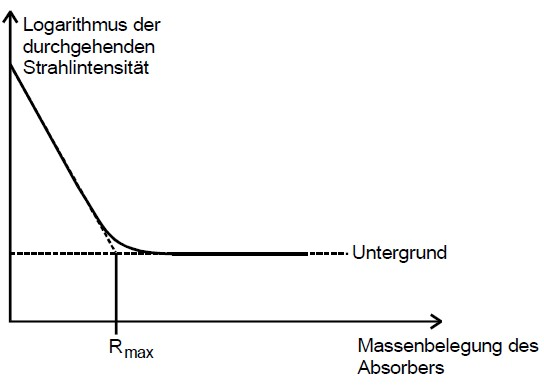
\includegraphics[height=6cm]{content/pics/beta_absorption.jpg}
    \caption{Absorptionskurve eines $\beta$-Strahlers \cite{v704}.}
    \label{fig:beta_abs}
\end{figure}
Im Allgemeinen lässt sich aus der Kurve die maximale Reichweite $R_{\text{max}}$ ablesen, indem der Schnittpunkt
der Geraden mit dem Untergrund gebildet wird.
Die beim $\beta$-Zerfall frei werdende Gesamtenergie $E_{\text{max}}$ lässt sich dann über folgenden empirischen
Zusammenhang aus $R_{\text{max}}$ bestimmen:
\begin{equation}
    \label{e_max}
    E_{\text{max}} = 1,92\sqrt{R_{\text{max}}^2 + 0,22R_{\text{max}}}.
\end{equation}

\subsection{\texorpdfstring{Absorption von $\gamma$-Strahlung}{Absorption von Gamma-Strahlung}}

Im Gegensatz zu $\beta$-Strahlung besitzt $\gamma$-Strahlung keine Ladung und nur eine relativistische Masse,
da sie aus Photonen besteht. Über die Quantentheorie lässt sich die Energie eines $\gamma$-Quants über
\begin{equation*}
    E_\gamma = hf = \frac{hc}{\lambda}
\end{equation*}
berechnen.
Beim Eindringen in eine Materieschicht können die $\gamma$-Quanten mit dem Atomkernen und deren elektrischen Feldern
sowie den Atomelektronen wechselwirken.
Bei jeder dieser Interaktionen kann es zu Annihilationen, Energieverlusten sowie Richtungsänderungen kommen,
insgesamt ist also eine große Vielfalt an Prozessen möglich.
Bei den \textbf{Annihilationsprozessen} verschwindet das $\gamma$-Quant, bei \textbf{inelastischer Streuung}
ändert es seine Richtung und gibt einen Teil seiner Energie ab, während bei \textbf{elastischer Streuung} nur
eine Richtungsänderung auftritt.
In \autoref{fig:gamma_abs} sind alle möglichen Prozesse übersichtlich in einer Tabelle dargestellt.
\begin{figure}[H]
    \centering
    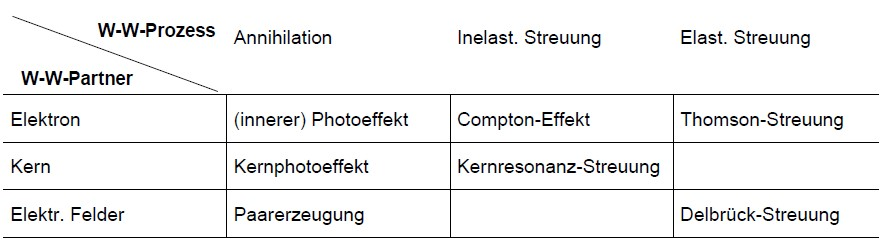
\includegraphics[height=4cm]{content/pics/gamma_absorption.jpg}
    \caption{Tabelle mit den verschiedenen Wechselwirkungen von $\gamma$-Strahlung mit Materie \cite{v704}.}
    \label{fig:gamma_abs}
\end{figure}
Die drei wichtigsten Prozesse sind der Photo-Effekt, Compton-Effekt und die Paarerzeugung, sie sollen im
Folgenden Näher betrachtet werden.
\begin{itemize}
    \item Beim (inneren) \textbf{Photo-Effekt} wechselwirkt ein $\gamma$-Quant mit einem Hüllenelektron.
    Dabei wird der $\gamma$-Quant vernichtet und das Elektron aus seiner Bindung entfernt.
    Das Elektron erhält also eine kinetische Energie gemäß
    \begin{equation*}
        E_{\symup{e}} = h\nu - E_{\symup{B}}
    \end{equation*}
    wobei $\nu$ die Frequenz des beteiligten $\gamma$-Quants ist. Man sieht sofort,das dieser Effekt nur
    auftreten kann, wenn $h\nu > E_{\symup{B}}$ ist.
    Der Photo-Effekt ist begleitet durch die Emmission von Röntgenquanten oder Auger-Elektronen, die durch
    ein Auffüllen der entstandenen Lücken durch Elektronen aus höheren Schalen verursacht werden.
    Über den Wirkungsquerschnitt lässt sich hier sagen, dass dieser bezogen auf $K$-Elektronen
    proportional zu $Z^5$ und $E_\gamma^{-3.5}$ ist.

    \item Als nächstes wird der \textbf{Compton-Effekt} behandelt, er beschreibt die Streuung eines
    $\gamma$-Quants an einem freien Elektron, beispielsweise an einem Leitungselektron im Metall.
    Hierbei wird die Richtung sowie die Energie des $\gamma$-Quants verändert, aber die Quanten können
    niemals verschwinden. Die Streuung der Quanten führt zu einer Intensitätsabnahme der $\gamma$-Strahlung.
    Für kleine Energien $(E_\gamma \ll m_0 \symup{c}^2)$ geht der Wirkungsquerschnitt $\sigma_{\text{Co}}$
    in dem Thomschonschen Wirkungsquerschnitt über, der durch
    \begin{equation}
        % \label{sigma_th}
        \sigma_{\symup{Th}} = \frac{8}{3}\pi \symup{r_e}^2 \notag
    \end{equation}
    gegeben ist.

    \item Zuletzt wird die \textbf{Paarerzeugung} beschrieben, die nur bei $E_\gamma > 2m_0 \symup{c}^2$ auftreten kann.
    Bei diesem Effekt spaltet sich ein $\gamma$-Quant in ein Elektron und ein Positron auf.
    Damit neben der Energieerhaltung auch die Impulserhaltung erfüllt ist, muss ein Teil des Quantenimpulses von
    einem weiteren Stoßpartner übernommen werden. In Absorbermaterialien bieten sich dafür die Atomkerne an,
    weshalb die Paarerzeugung im Coulombfeld der Atomkerne auftritt.
    Für den Wirkungsquerschnitt gilt hier $\sigma_{\text{p}} \sim \symup{z}^2$.
\end{itemize}

Bei der Absorption von $\gamma$-Strahlung überlagern sich all diese Prozesse, ihre Gewichtung hängt stark von der
Energie der $\gamma$-Strahlung sowie dem Material ab.
Bei niedrigen Energien dominiert der Photo-Effekt, der Compton-Effekt spielt erst bei mittleren Energien eine Rolle.
Die Paarerzeugung setzt erst bei hohen Energien um etwa $\qty{1}{\mega\electronvolt}$ ein, dominiert dann aber
ab $\qty{100}{\mega\electronvolt}$ nahezu vollständig.